%% LyX 2.3.3 created this file.  For more info, see http://www.lyx.org/.
%% Do not edit unless you really know what you are doing.
\documentclass[american]{article}
\usepackage{lmodern}
\usepackage[latin9]{inputenc}
\usepackage[a4paper]{geometry}
\geometry{verbose,tmargin=1cm,bmargin=4cm,lmargin=3cm,rmargin=3cm}
\usepackage{color}
\usepackage{graphicx}
\usepackage[authoryear]{natbib}

\makeatletter
%%%%%%%%%%%%%%%%%%%%%%%%%%%%%% User specified LaTeX commands.
\usepackage[usenames,dvipsnames,svgnames,table]{xcolor}

\makeatother

\usepackage{babel}
\usepackage{listings}
\lstset{basicstyle={\footnotesize\bfseries\ttfamily},
breaklines=true,
commentstyle={\itshape\color{OliveGreen}},
keywordstyle={\bfseries\color{blue}},
showstringspaces=true,
stringstyle={\bfseries\color{RoyalPurple}}}
\begin{document}
\title{Advanced radiation and remote sensing }
\author{Lukas Kluft, Manfred Brath, Stefan B�hler}
\maketitle

\subsection*{Exercise No. 6 -- Inversion theory: Optimal Estimation Method (OEM)}

In this exercise you will work with \textquotedblleft realistic\textquotedblright{}
data measured by a water vapor radiometer. The data is not real but
has been simulated for a well-known atmospheric state using ARTS.
Simulated measurements allow to compare retrieval results to the true
atmospheric state. The radiometer (Fig. 1) measures thermal radiation
in a frequency range around the 22 GHz water vapor absorption line.
As the pressure broadening of absorption lines varies with height
the measurement contains information about the vertical water vapor
profile. This information can be retrieved using the \textquotedblleft Optimal
Estimation Method\textquotedblright{} (OEM). The radiometer is placed
in 10 km height, which resembles an upward looking airborne measurement.
The scarce concentration of water vapor in the stratosphere allows
to perform a linear retrieval approach. Retrievals that cover the
whole atmosphere, including the highly absorbent lower troposphere,
need more advanced retrieval approaches like an iterative OEM. 
\begin{figure}
\centerline{ 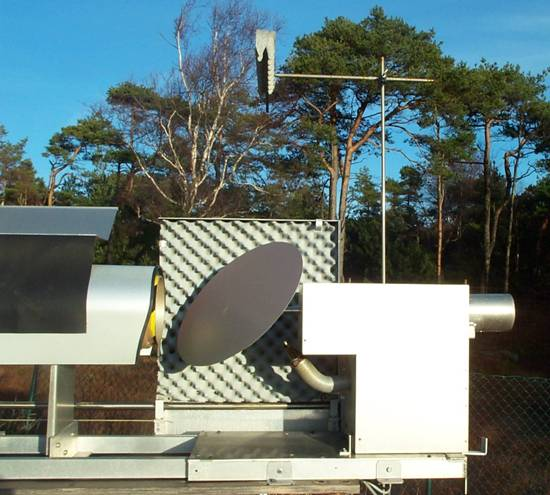
\includegraphics[width=7cm]{H2Orad} }\caption{\label{fig:onsala} Onsala water vapor radiometer (photo: Peter Forkman)}
\end{figure}

\begin{enumerate}
\item Run the Python script \texttt{oem.py} and plot the observed brightness
temperature spectrum \texttt{y\_measurement} as function of frequency
\texttt{f\_grid}.
\item Uncomment the line with the function call \texttt{forward\_model()}
and rerun the script to simulate the brightness temperature spectrum
\texttt{y} and the water vapor Jacobian \texttt{K} for the \emph{a
priori} state.
\begin{enumerate}
\item Add the simulated brightness temeperature spectrum to the plot of
the observed brightness temperature spectrum.
\item Plot the Jacobians \texttt{K} in a suitable way. Explain the plot.
\end{enumerate}
\item Plot the measurement covariance matrix \texttt{S\_y} and the \emph{a
priori} covariance matrix \texttt{S\_xa} in a suitable way. What do
the covariance matrices mean?
\item Implement the function \texttt{retrieve()} according to the OEM solution:
\begin{equation}
\hat{\mathbf{x}}=\mathbf{x}_{a}+\left(\mathbf{K}^{T}\mathbf{S}_{y}^{-1}\mathbf{K}+\mathbf{S}_{xa}^{-1}\right)\mathbf{K}^{T}\mathbf{S}_{y}^{-1}\left(\mathbf{y}_{measure}-\mathbf{y}_{a}\right)
\end{equation}
 with $\mathbf{x}_{a}$ the a priori profile, $\mathbf{K}$ the Jacobian,
$\mathbf{S}_{y}$ the measurement covariance matrix, $\mathbf{S}_{xa}$
the \emph{a priori} covariance matrix, $\mathbf{y}_{measure}$ the
observed brightness temperature spectrum and $\mathbf{y}_{a}$ the
simulated brightness temperature spectrum of profile $\mathbf{x}_{a}$.

In Python, a matrix \texttt{M} can be transposed using \texttt{M.T}
and inversed using \texttt{inv(M)}\footnote{We are using the inverse function \texttt{scipy.linalg.inv() }provided
by the SciPy package.}. Two matrices \texttt{M1} and \texttt{M2} can be multiplied using
\texttt{M1 @ M2.}
\item Use the function \texttt{retrieve()} to retrieve the water vapor profile.
\item Plot the retrieved water vapor \texttt{x\_oem} and the \emph{a priori}
water vapor profile as function of height~\texttt{z}.
\item Load the true water vapor retrieval (\texttt{input/x\_true.xml}) and
add it to the previous plot. Dicuss the results.
\item Implement the function \texttt{averaging\_kernel\_matrix() }to calculate
the same-named matrix:
\begin{equation}
\mathbf{A}=\left(\mathbf{K}^{T}\mathbf{S}_{y}^{-1}\mathbf{K}+\mathbf{S}_{xa}^{-1}\right)\mathbf{K}^{T}\mathbf{S}_{y}^{-1}\mathbf{K}
\end{equation}
\item Plot the kernels (columns) of $\mathbf{A}$ as function of height
\texttt{z} and interpret the results.
\item The measurement response is defined as the sum over all averaging
kernels in a given height (row). The measurement response indicates
in which heights the measurement actually adds information to the
retrieval result. 
\begin{enumerate}
\item Calculate the measurement response and plot it together with the averaging
kernels. 
\item In which heights does the measurement provide useful information? 
\item Is it possible to estimate the vertical resolution?
\end{enumerate}
\end{enumerate}

\end{document}
